\documentclass[journal,12pt,twocolumn]{IEEEtran}
\usepackage{amsmath,amssymb,amsfonts,amsthm}
\usepackage{txfonts}
\usepackage{tkz-euclide}
\usepackage{listings}
\usepackage{gvv}
\usepackage[latin1]{inputenc}
\usepackage{adjustbox}
\usepackage{array}
\usepackage{tabularx}
\usepackage{enumitem}
\usepackage{pgf}
\usepackage{lmodern}
\usepackage{circuitikz}
\usepackage{tikz}
\usepackage{graphicx}


\begin{document}
\bibliographystyle{IEEEtran}

\vspace{3cm}

\title{}
\author{EE23BTECH11054 -  Sai Krishna Shanigarapu$^{*}$
}
\maketitle
\newpage
\bigskip

\section*{Gate EE 2022}
28. \hspace{2pt}The network shown below has a resonant frequency of 150 kHz and bandwidth of 600
Hz. The Q-factor of the network is \rule{1cm}{0.15mm}\\
(rounded off to one decimal place).\\
\hfill(GATE 2022 EC)\\
\begin{figure}[ht]
  \centering
  %\begin{adjustbox}{width=\columnwidth}
      \begin{circuitikz}[american]
    \draw (0,0) to [short, *-] (5,0) to [R=R] (5,2) to [L=L] (5,4) to [short] (2,4) to [C=C] (2,0);
    \draw (0,4) to [short, *-] (2,4);
\end{circuitikz}
  %\end{adjustbox}
  \caption{Circuit 1}
\end{figure}\\
\solution\\

\begin{table}[ht]
    \centering
    \begin{adjustbox}{width=\columnwidth}
    \setlength{\arrayrulewidth}{0.3mm}
\setlength{\tabcolsep}{20pt}
\renewcommand{\arraystretch}{1.3}


\begin{tabular}{|c|c|c|}
\hline
Parameter & Description & Value\\
\hline
$f_0$ & Resonant frequency & 150 kHz\\
\hline
$B$ & Bandwidth & 600 Hz\\
\hline
$Q$ & Quality factor & ?\\
\hline
\end{tabular}
    \end{adjustbox}
    \caption{Parameters}
    \label{tab:tab1_gate_ee_2022_28_054}
\end{table}
%Using Table \ref{tab:tab1_gate_ee_2022_28_054},
\begin{align}
    Q &= \frac{f_0}{B}\\
    &=\frac{150 \text{ x } 10^3}{600}\\
    &= 250
\end{align}

$\therefore$ Q-factor is 250

\begin{figure}
    \centering
    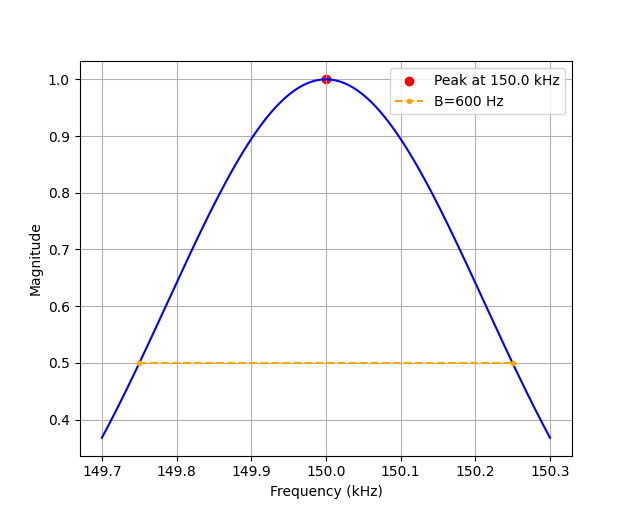
\includegraphics[width=\columnwidth]{figs/Figure_1.png}
    \caption{Plot of Q-factor}
    \label{fig:fig1_gate_ee_2022_18_054}
\end{figure}

\end{document}
